\begin{figure}[h]
  \begin{center}
    \begin{adjustbox}{width=0.5\columnwidth}

        \tikzset{every picture/.style={line width=0.75pt}}       
        
        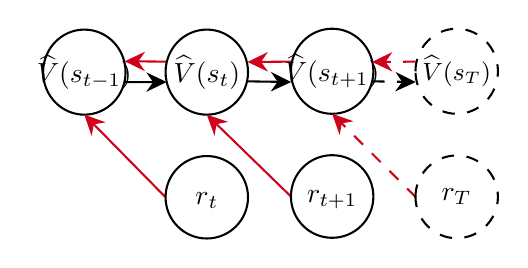
\begin{tikzpicture}[x=0.75pt,y=0.75pt,yscale=-1,xscale=1]
        
        %Straight Lines [id:da2592063600931961] 
        \draw [color={rgb, 255:red, 208; green, 2; blue, 27 }  ,draw opacity=1 ]   (282.5,135.16) -- (300.67,135.02) ;
        \draw [shift={(279.5,135.18)}, rotate = 359.55] [fill={rgb, 255:red, 208; green, 2; blue, 27 }  ,fill opacity=1 ][line width=0.08]  [draw opacity=0] (9.82,-4.72) -- (0,0) -- (9.82,4.72) -- (6.52,0) -- cycle    ;
        %Straight Lines [id:da41585806917853485] 
        \draw [color={rgb, 255:red, 208; green, 2; blue, 27 }  ,draw opacity=1 ]   (223.33,134.87) -- (240.67,135.02) ;
        \draw [shift={(220.33,134.85)}, rotate = 0.47] [fill={rgb, 255:red, 208; green, 2; blue, 27 }  ,fill opacity=1 ][line width=0.08]  [draw opacity=0] (9.82,-4.72) -- (0,0) -- (9.82,4.72) -- (6.52,0) -- cycle    ;
        %Shape: Ellipse [id:dp31493856088290983] 
        \draw   (181,140.07) .. controls (181,128.75) and (189.89,119.58) .. (200.86,119.58) .. controls (211.83,119.58) and (220.72,128.75) .. (220.72,140.07) .. controls (220.72,151.4) and (211.83,160.57) .. (200.86,160.57) .. controls (189.89,160.57) and (181,151.4) .. (181,140.07) -- cycle ;
        %Shape: Ellipse [id:dp5103941395609547] 
        \draw  [dash pattern={on 4.5pt off 4.5pt}] (360.4,139.66) .. controls (360.4,128.34) and (369.29,119.16) .. (380.26,119.16) .. controls (391.23,119.16) and (400.12,128.34) .. (400.12,139.66) .. controls (400.12,150.98) and (391.23,160.16) .. (380.26,160.16) .. controls (369.29,160.16) and (360.4,150.98) .. (360.4,139.66) -- cycle ;
        %Straight Lines [id:da30559831832260953] 
        \draw [color={rgb, 255:red, 0; green, 0; blue, 0 }  ,draw opacity=1 ]   (220.07,144.9) -- (237.5,144.86) ;
        \draw [shift={(240.5,144.85)}, rotate = 539.86] [fill={rgb, 255:red, 0; green, 0; blue, 0 }  ,fill opacity=1 ][line width=0.08]  [draw opacity=0] (9.82,-4.72) -- (0,0) -- (9.82,4.72) -- (6.52,0) -- cycle    ;
        %Shape: Ellipse [id:dp12377292733336898] 
        \draw  [color={rgb, 255:red, 0; green, 0; blue, 0 }  ,draw opacity=1 ] (240,140.07) .. controls (240,128.75) and (248.89,119.58) .. (259.86,119.58) .. controls (270.83,119.58) and (279.72,128.75) .. (279.72,140.07) .. controls (279.72,151.4) and (270.83,160.57) .. (259.86,160.57) .. controls (248.89,160.57) and (240,151.4) .. (240,140.07) -- cycle ;
        %Shape: Ellipse [id:dp9248757796917767] 
        \draw   (300.4,139.66) .. controls (300.4,128.34) and (309.29,119.16) .. (320.26,119.16) .. controls (331.23,119.16) and (340.12,128.34) .. (340.12,139.66) .. controls (340.12,150.98) and (331.23,160.16) .. (320.26,160.16) .. controls (309.29,160.16) and (300.4,150.98) .. (300.4,139.66) -- cycle ;
        %Straight Lines [id:da050274800713848156] 
        \draw [color={rgb, 255:red, 208; green, 2; blue, 27 }  ,draw opacity=1 ]   (202.96,162.71) -- (240,200.37) ;
        \draw [shift={(200.86,160.57)}, rotate = 45.48] [fill={rgb, 255:red, 208; green, 2; blue, 27 }  ,fill opacity=1 ][line width=0.08]  [draw opacity=0] (9.82,-4.72) -- (0,0) -- (9.82,4.72) -- (6.52,0) -- cycle    ;
        %Straight Lines [id:da7059353635730191] 
        \draw [color={rgb, 255:red, 208; green, 2; blue, 27 }  ,draw opacity=1 ]   (262.01,162.66) -- (300.4,200) ;
        \draw [shift={(259.86,160.57)}, rotate = 44.2] [fill={rgb, 255:red, 208; green, 2; blue, 27 }  ,fill opacity=1 ][line width=0.08]  [draw opacity=0] (9.82,-4.72) -- (0,0) -- (9.82,4.72) -- (6.52,0) -- cycle    ;
        %Straight Lines [id:da17885982011746426] 
        \draw [color={rgb, 255:red, 208; green, 2; blue, 27 }  ,draw opacity=1 ] [dash pattern={on 4.5pt off 4.5pt}]  (322.38,162.28) -- (360.4,200.16) ;
        \draw [shift={(320.26,160.16)}, rotate = 44.9] [fill={rgb, 255:red, 208; green, 2; blue, 27 }  ,fill opacity=1 ][line width=0.08]  [draw opacity=0] (9.82,-4.72) -- (0,0) -- (9.82,4.72) -- (6.52,0) -- cycle    ;
        %Shape: Ellipse [id:dp3523005799699832] 
        \draw  [dash pattern={on 4.5pt off 4.5pt}] (360.4,200.16) .. controls (360.4,189.16) and (369.29,180.23) .. (380.26,180.23) .. controls (391.23,180.23) and (400.12,189.16) .. (400.12,200.16) .. controls (400.12,211.17) and (391.23,220.09) .. (380.26,220.09) .. controls (369.29,220.09) and (360.4,211.17) .. (360.4,200.16) -- cycle ;
        %Shape: Ellipse [id:dp3509500153089894] 
        \draw   (300.4,200) .. controls (300.4,189) and (309.29,180.09) .. (320.26,180.09) .. controls (331.23,180.09) and (340.12,189) .. (340.12,200) .. controls (340.12,210.99) and (331.23,219.9) .. (320.26,219.9) .. controls (309.29,219.9) and (300.4,210.99) .. (300.4,200) -- cycle ;
        %Shape: Ellipse [id:dp17336392317383575] 
        \draw  [color={rgb, 255:red, 0; green, 0; blue, 0 }  ,draw opacity=1 ] (240,200.37) .. controls (240,189.4) and (248.89,180.5) .. (259.86,180.5) .. controls (270.83,180.5) and (279.72,189.4) .. (279.72,200.37) .. controls (279.72,211.34) and (270.83,220.23) .. (259.86,220.23) .. controls (248.89,220.23) and (240,211.34) .. (240,200.37) -- cycle ;
        %Straight Lines [id:da21459790152477998] 
        \draw [color={rgb, 255:red, 0; green, 0; blue, 0 }  ,draw opacity=1 ]   (279.5,144.52) -- (297.5,144.8) ;
        \draw [shift={(300.5,144.85)}, rotate = 180.91] [fill={rgb, 255:red, 0; green, 0; blue, 0 }  ,fill opacity=1 ][line width=0.08]  [draw opacity=0] (9.82,-4.72) -- (0,0) -- (9.82,4.72) -- (6.52,0) -- cycle    ;
        %Straight Lines [id:da8588950475203374] 
        \draw [color={rgb, 255:red, 208; green, 2; blue, 27 }  ,draw opacity=1 ] [dash pattern={on 4.5pt off 4.5pt}]  (342.5,135.16) -- (360.67,135.02) ;
        \draw [shift={(339.5,135.18)}, rotate = 359.55] [fill={rgb, 255:red, 208; green, 2; blue, 27 }  ,fill opacity=1 ][line width=0.08]  [draw opacity=0] (9.82,-4.72) -- (0,0) -- (9.82,4.72) -- (6.52,0) -- cycle    ;
        %Straight Lines [id:da9169375689094925] 
        \draw [color={rgb, 255:red, 0; green, 0; blue, 0 }  ,draw opacity=1 ] [dash pattern={on 4.5pt off 4.5pt}]  (339.5,144.52) -- (357.5,144.8) ;
        \draw [shift={(360.5,144.85)}, rotate = 180.91] [fill={rgb, 255:red, 0; green, 0; blue, 0 }  ,fill opacity=1 ][line width=0.08]  [draw opacity=0] (9.82,-4.72) -- (0,0) -- (9.82,4.72) -- (6.52,0) -- cycle    ;
        
        % Text Node
        \draw (320.26,201.59) node    {$r_{t+1}$};
        % Text Node
        \draw (200.86,140.07) node    {$\widehat{V}(s_{t-1})$};
        % Text Node
        \draw (320.26,139.66) node    {$\widehat{V}(s_{t+1})$};
        % Text Node
        \draw (380.26,139.66) node  [font=\small]  {$\widehat{V}(s_{T})$};
        % Text Node
        \draw (259.86,202) node  [color={rgb, 255:red, 208; green, 9; blue, 2 }  ,opacity=1 ]  {$\textcolor[rgb]{0,0,0}{r}\textcolor[rgb]{0,0,0}{_{t}}$};
        % Text Node
        \draw (259.86,140.07) node  [color={rgb, 255:red, 208; green, 9; blue, 2 }  ,opacity=1 ]  {$\textcolor[rgb]{0,0,0}{\widehat{V}}\textcolor[rgb]{0,0,0}{(s_{t})}$};
        % Text Node
        \draw (380.26,200.16) node    {$r_{T}$};

        \end{tikzpicture}
    \end{adjustbox}
  \end{center}
\caption{\textbf{Graphical representation of TD Learning}. Red arrows indicate the flow of the computations for deriving $\delta$ and updating $\widehat{V}$ expressed by equations \ref{td_error} and \ref{td_update}. Black arrows instead indicate the changes of $\widehat{V}$ moving from $s$ to $s_{t+1}$. Solid circles indicate states which have already been observed while dashed ones represent future not-yet observed states.}
\label{fig: td_learning}
\end{figure}